\section{Our model}
\begin{frame}
\frametitle{RNN Encoder-decoder}
\begin{columns}
\begin{column}{0.65\textwidth}
\begin{itemize}
\item Recurrent neural network composed of sequentially ordered cells
\item Maintains (encodes) hidden state and emits observation after each turn
\item Improved with LSTM cells
\item Suitable for DST task - history is taken into account
\end{itemize}
\end{column}
\begin{column}{0.35\textwidth}
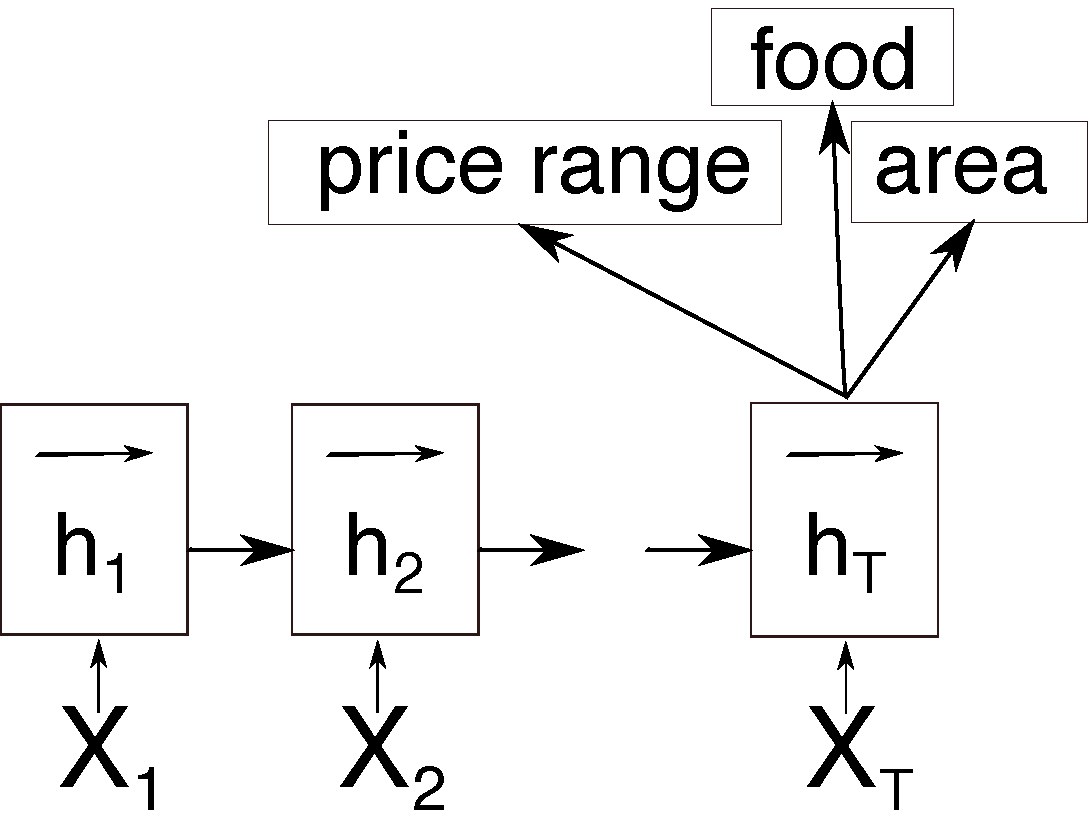
\includegraphics[width=0.90\textwidth]{encoder.pdf}
\end{column}
\end{columns}
\end{frame}

\begin{frame}
\frametitle{Model details}
\begin{itemize}
\item TensorFlow framework - good performance and desired functionality, e.g. GPU computation, \texttt{seq2seq}
\item Supervised learning
\item Predicting labels jointly or independently
\begin{itemize}
\item joint model suffers from data sparsity\
\end{itemize}
\end{itemize}
\end{frame}

\begin{frame}
\frametitle{Model details}
\begin{itemize}
\item INPUT FEATURES
\begin{itemize}
\item one-hot encoding (Bag of Words)
\item vector embeddings of words
\item indicator, whether the word belong to particular domain 
\end{itemize}
\item We do not predict the method - trivial
\end{itemize}
\end{frame}

\begin{frame}
\frametitle{Training and Evaluation}
\begin{itemize}
\item During training, each turn is predicted based on whole dialogue history
\item Data separated into buckets of similar lengths 
\item \textbf{Accuracy} metric was used, i.e. fraction of turns, where the most probable hypotheses was correct
\item \textbf{schedule 2} includes only turns, where some information is taken from the user
\end{itemize}
\end{frame}